\providecommand{\topdir}{..}
\documentclass[../main.tex]{subfiles}

%External sources
\graphicspath{{\topdir/img/07/}}

\begin{document}
\label{chap:future}

This project provides a good baseline for developing related projects on top. These projects can be classified in two groups: The expansion of the capabilities of the mixer itself and the development of controllers for the mixer.\newline

\section{Expansion and improvement of the mixer}
As described earlier, the architecture of the mixer allows easy expansion by inheriting from the provided base classes. The most important base classes that have a high potential of expansion are \texttt{ZuazoBase}, \texttt{TransitionBase} and \texttt{OverlayBase}.\newline

\subsection{Adding new video processing elements}
Currently, the fan of available video processors is very narrow, as there are only four classes that perform such a task (the media player, the \gls{ndi} source, the window output and the \gls{me}). However, inheriting from the \texttt{ZuazoBase} class, new elements can be added. Here are some useful examples of them:\newline

\subsubsection{Mosaic viewer}
All modern mixers, regardless of their implementation, integrate a component that allows to simultaneously view multiple sources at the same time. This component is commonly referred as the mosaic generator or the multi-viewer. Moreover, they usually show useful information such as a signal identifier and a tally light. Adding a plain mosaic viewer is an easy task using the \textit{Zuazo} library. In fact, at the current state, a \gls{me} could be configured to accomplish this task. However, adding the tally light and especially the text requires a bit more of effort.\newline

\subsubsection{Colour-bar generators}
As the name suggests, it would be useful to have a component that procedurally generates standard color bars. These color bars can be used to test many aspects of the mixer.\newline

\subsubsection{NDI output}
Currently, only \gls{ndi} input is implemented. However, this protocol also allows outputting video, which might be useful for many production environments. Implementing this feature would involve expanding the \textit{zuazo-ndi} module and wrapping it with a mixer component.\newline

\subsubsection{SDI I/O through Black Magick Design's DeckLink cards}
Similarly to the previous improvement, this one also involves expanding the \gls{io} capabilities of the mixer. In this case, the new \gls{io} would be performed using \gls{sdi} through Black Magick's DeckLink cards. These cards offer a good cross-platform C++ programming \gls{api}.\newline

\subsection{Improvements to existing video processing elements}
Some existing elements have plenty of room for improvement. For instance, the control of the media players is very rudimentary. Important features like entry points, playlists and synchronization are missing.\newline

\subsection{Adding new transitions}
Similarly to the expansion of video processing elements, new transitions can be added by inheriting from \texttt{TransitionBase}. Currently, wipe style transitions have not been implemented, so there is definitely room for improvement. Moreover, the existing transitions can be further improved by adding more variations.\newline

\section{Development and improvement of controllers}
As mentioned in previous chapters, the mixer itself is agnostic of the \gls{ui}. This allows to implement different controllers that focus on different usages of a production switcher. Some examples of controllers are described hereafter.\newline

\subsection{Physical control panel}
Although in the \autoref{chap:control} a prototype of a physical panel is described, this is a mere proof of concept. Moreover, the physical control panel lacks some of the most crucial aspects such as the \textit{t-bar}. However this prototype proofs the viability of implementing a control panel that interacts with this mixer.\newline

There are two strategies to accomplish this task. The first one is to design everything from scratch. The benefit of doing so is that everything is under the control of the designer, but it requires a lot of work. The other approach is to reverse engineer a decommissioned commercial control panel to adapt it to the new mixer.\newline

\subsection{Improvements of the web application based controller}
Although the implemented web application for controlling the mixer covers most aspects of it, there is a lot of room for improvement. 

\subsection{Show sequencer}
Another interesting controller would be a sequencer. Unlike all previous controllers, this does not require a human operator. Instead, the camera shots are time-coded. In essence, linear \gls{tv} is produced as if it were nonlinear. Currently, the only application that allows to do this is CuePilot, which is shown in the figure \ref{fig:07:cuepilot}. The multi-client nature of this mixer is ideal for this type of control, as a human controller can override the automated controls.

\begin{figure}[htbp]
    \centering
    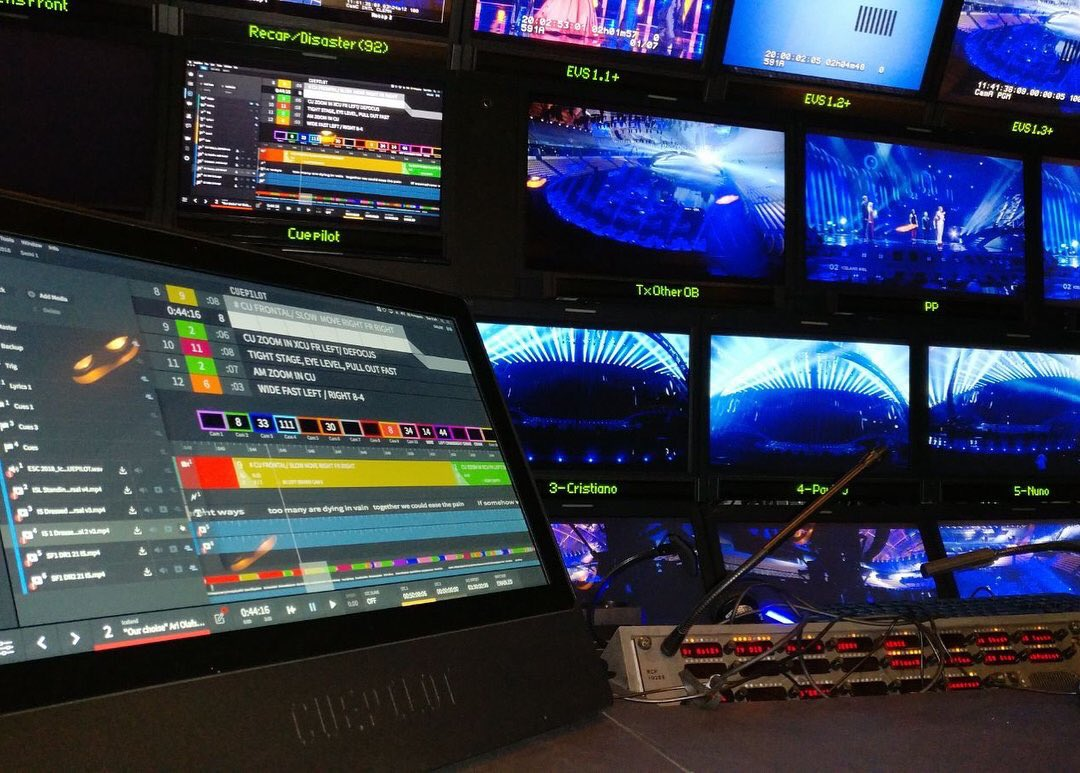
\includegraphics[width=.8\textwidth]{CuePilot}
    \caption{CuePilot being used at the Eurovision Song Contest 2017}
    \label{fig:07:cuepilot}
\end{figure}

%Print bibliography if it is being compiled standalone
%\printbibliography

\end{document}
